% ======================================================================
%  CMPT 225 -- Assignment 1
%  Total: 123 marks in 9 parts (A--I).
%  Compile with pdflatex, twice, so that "Page x of y" resolves.
% ======================================================================
\documentclass[11pt]{article}

\usepackage[letterpaper, margin=1in, headheight=14pt]{geometry}
\usepackage{microtype}
\usepackage{amsmath, amssymb}
\usepackage{array, booktabs, tabularx}
\usepackage{enumitem}
\usepackage{xcolor}
\usepackage{listings}
\usepackage{tikz}
\usetikzlibrary{positioning}
\usepackage{fancyhdr}
\usepackage{lastpage}
\usepackage{needspace}

% ------------------------------------------------------------------ page
\pagestyle{fancy}
\fancyhf{}
\fancyhead[L]{\small CMPT 225 --- Assignment 1}
\fancyfoot[C]{\small Page \thepage\ of \pageref{LastPage}}
\fancypagestyle{cover}{\fancyhf{}%
  \fancyfoot[C]{\small Page \thepage\ of \pageref{LastPage}}%
  \renewcommand{\headrulewidth}{0pt}}
\setlength{\parindent}{0pt}
\setlength{\parskip}{4pt}

% ------------------------------------------------------------------ code
\lstset{
  language=Java,
  basicstyle=\ttfamily\small,
  keywordstyle=,
  commentstyle=\itshape,
  columns=fullflexible,
  keepspaces=true,
  showstringspaces=false,
  frame=single,
  rulecolor=\color{black!40},
  framesep=5pt,
  xleftmargin=1.5em,
  xrightmargin=1.5em,
  aboveskip=8pt,
  belowskip=8pt
}
\newcommand{\code}[1]{\mbox{\texttt{#1}}}  % never split inline code across lines
\newcommand{\lb}{\char`\{}   % typewriter braces for use inside \code
\newcommand{\rb}{\char`\}}

% ----------------------------------------------------------------- marks
% \score{m} puts the marker's box "[   / m ]" at the right margin, at the
% end of a paragraph. In every Part, the boxes add up to the Part total.
\newcommand{\score}[1]{{\unskip\nobreak\hfil\penalty50
  \hskip2em\hbox{}\nobreak\hfil\mbox{[\hspace{2.5em}/\,#1\,]}%
  \parfillskip=0pt \finalhyphendemerits=0 \par}}
\newcommand{\cellscore}[1]{\mbox{[\hspace{2.5em}/\,#1\,]}}

% \partheading[keep]{letter}{title}{marks}   \question[keep]{label}{title}{marks}
% The optional [keep] is the space kept together with the heading, so that a
% short question is not split across two pages.
\newcommand{\partheading}[4][12\baselineskip]{\needspace{#1}%
  \section*{Part #2 --- #3\hfill{\normalsize\normalfont(#4 marks)}}}
\newcommand{\question}[4][8\baselineskip]{\needspace{#1}%
  \subsection*{#2.\ #3\hfill{\normalsize\normalfont(#4 marks)}}}

\setlist[enumerate,1]{label=\textbf{(\alph*)}, leftmargin=2.2em,
  itemsep=5pt, topsep=4pt}
\setlist[itemize]{itemsep=1pt, topsep=2pt}
\newcolumntype{C}[1]{>{\centering\arraybackslash}p{#1}}
\newcolumntype{L}[1]{>{\raggedright\arraybackslash}p{#1}}
\newcolumntype{Y}{>{\raggedright\arraybackslash}X}

\begin{document}

% ================================================================= COVER
\thispagestyle{cover}
\begin{center}
  {\LARGE\bfseries CMPT 225 --- Assignment 1\par}
  \medskip
  {\large Total: 123 marks \,$\cdot$\, 9 parts (A--I)\par}
\end{center}

\bigskip
\begin{tabular}{@{}l p{10cm}@{}}
  \textbf{Student Name:} & \hrulefill \\[16pt]
  \textbf{Student ID:}   & \hrulefill \\
\end{tabular}

\subsection*{Rules}
\begin{itemize}
  \item Code may be written in Java or in clear Java-like pseudocode.
  \item Use only the library classes a question explicitly allows.
  \item Show your work.
\end{itemize}

\subsection*{Conventions}
Unless a question states otherwise, the following conventions hold.
\begin{itemize}
  \item $n$ is the input size.
  \item $\log$ means $\log_2$.
  \item ``Running time'' means worst-case running time.
  \item ``Space'' means auxiliary space: memory used beyond the input,
        including the function call stack.
  \item ``Tightest bound'' means give a $\Theta$ bound.
  \item Draw linked structures as boxes and arrows.
  \item Represent a \code{null} reference as $\varnothing$.
\end{itemize}

\subsection*{Grading}
\begin{center}
\renewcommand{\arraystretch}{1.4}
\begin{tabular}{|c|l|r|C{2.8cm}|}
  \hline
  \textbf{Part} & \textbf{Topic} & \textbf{Marks} & \textbf{Score} \\ \hline
  A & Asymptotic notation: concepts & 24 & \\ \hline
  B & Asymptotic notation: proofs   & 12 & \\ \hline
  C & Analyzing time and space      & 15 & \\ \hline
  D & Singly linked lists           & 18 & \\ \hline
  E & Doubly linked lists           & 18 & \\ \hline
  F & Stacks                        & 17 & \\ \hline
  G & Queues                        &  6 & \\ \hline
  H & The function call stack       &  5 & \\ \hline
  I & Design problems               &  8 & \\ \hline
    & \textbf{Total}                & \textbf{123} & \\ \hline
\end{tabular}
\end{center}

\clearpage

% ================================================================ PART A
\partheading{A}{Asymptotic Notation: Concepts}{24}

\question{A1}{Definitions}{6}
Let $f(n)$ and $g(n)$ be functions from the positive integers to the
non-negative real numbers.
\begin{enumerate}
  \item State the formal definition of $f(n) \in O(g(n))$. \score{2}
  \vspace{3cm}
  \item State the formal definition of $f(n) \in \Omega(g(n))$. \score{2}
  \vspace{3cm}
  \item State the formal definition of $f(n) \in \Theta(g(n))$. In one
        sentence, explain what a $\Theta$ bound tells you that an $O$ bound
        alone does not. \score{2}
    \vspace{3cm}
\end{enumerate}

\question[14\baselineskip]{A2}{True or false?}{12}
For each statement, write \textbf{T} or \textbf{F} and justify it in one or
two lines (a short calculation, a pair of constants, or a counterexample).
Each part is worth 1.5 marks: 0.5 for the verdict and 1 for the
justification.
\begin{enumerate}
  \item $3n^2 + 100n + 7 \in O(n^2)$ \score{1.5}
  \vspace{3cm}
  \item $n^2 \in O(n \log n)$ \score{1.5}
  \vspace{3cm}
  \item $2^{n+1} \in \Theta(2^n)$ \score{1.5}
  \vspace{3cm}
  \item $2^{2n} \in O(2^n)$ \score{1.5}
  \vspace{3cm}
  \item $\log_2 n \in \Theta(\log_{10} n)$ \score{1.5}
  \vspace{3cm}
  \item $(\log n)^3 \in O(n)$ \score{1.5}
  \vspace{3cm}
  \item If $f(n) \in O(g(n))$, then $g(n) \in \Omega(f(n))$. \score{1.5}
  \vspace{3cm}
  \item If an algorithm's worst-case running time is $\Theta(n^2)$, then it
        takes $\Omega(n^2)$ time on \emph{every} input of size $n$. \score{1.5}
  \vspace{3cm}
\end{enumerate}

\question[28\baselineskip]{A3}{Ranking growth rates}{6}
Rank the twelve functions below in order of increasing asymptotic growth rate, assigning rank 1 to the slowest-growing function or group of functions. Functions that are $\Theta$ of each other must receive the same rank and be listed in the same row, separated by commas. Assign consecutive ranks to distinct growth classes, with no gaps between ranks. \score{6}
\[
  n^2,\quad 4^{n/2},\quad n\log n,\quad 100,\quad \sqrt{n},\quad n!,\quad
  \log(n^2),\quad n^3/1000,\quad 2^n,\quad \log n,\quad n,\quad 2^{\log n}
\]
\begin{center}
\renewcommand{\arraystretch}{1.4}
\begin{tabular}{|c|L{11.5cm}|}
  \hline
  \textbf{Rank} & \textbf{Function(s)} \\ \hline
  1 (slowest) & \\ \hline
  2  & \\ \hline
  3  & \\ \hline
  4  & \\ \hline
  5  & \\ \hline
  6  & \\ \hline
  7  & \\ \hline
  8  & \\ \hline
  9  & \\ \hline
  10 & \\ \hline
  11 & \\ \hline
  12 & \\ \hline
\end{tabular}
\end{center}

% ================================================================ PART B
\partheading{B}{Asymptotic Notation: Proofs}{12}

Every proof in this Part must name explicit constants ($c$ and $n_0$, or
$c_1$, $c_2$ and $n_0$) and show that the required inequality holds for
\emph{all} $n \ge n_0$.

\question{B1}{A $\Theta$ proof}{8}
Let $f(n) = 5n^3 - 2n^2 + 8$.
\begin{enumerate}
  \item Prove that $f(n) \in O(n^3)$. \score{4}
  \vspace{3cm}
  \item Prove that $f(n) \in \Omega(n^3)$. \score{3}
  \vspace{3cm}
  \item Conclude that $f(n) \in \Theta(n^3)$, and state constants $c_1$,
        $c_2$ and $n_0$ that prove it. \score{1}
  \vspace{3cm}
\end{enumerate}

\question{B2}{The maximum rule}{4}
Let $f(n)$ and $g(n)$ be non-negative functions.
\begin{enumerate}
  \item Prove that $f(n) + g(n) \in \Theta(\max(f(n), g(n)))$. \score{3}
  \vspace{2cm}
  \item Use (a) to explain, in one or two sentences, why
        $n^3 + 1000n^2 \in \Theta(n^3)$, that is, why we may ``drop
        lower-order terms.'' \score{1}
\end{enumerate}

% ================================================================ PART C
\partheading{C}{Analyzing Time and Space}{15}

\question[17\baselineskip]{C1}{Code fragments}{12}
For each fragment, give the tightest bound on (i) the running time and
(ii) the auxiliary space, both as functions of $n$. Justify the running
time by showing the sum you used. Assume $n \ge 1$ and that \code{count} is
a \code{static int} field. Each fragment is worth 3 marks: 2 for the
running time with its justification and 1 for the space.

\medskip
\begin{minipage}[t]{0.48\textwidth}
\textbf{(a)} \score{3}
\begin{lstlisting}[xleftmargin=0pt, xrightmargin=0pt]
for (int i = 0; i < n; i++)
    for (int j = i; j < n; j++)
        count++;
\end{lstlisting}
\vspace{5cm}
\end{minipage}\hfill
\begin{minipage}[t]{0.48\textwidth}
\textbf{(b)} \score{3}
\begin{lstlisting}[xleftmargin=0pt, xrightmargin=0pt]
for (int i = 1; i <= n; i *= 2)
    for (int j = 0; j < i; j++)
        count++;
\end{lstlisting}
\vspace{5cm}
\end{minipage}

\medskip
\begin{minipage}[t]{0.48\textwidth}
\textbf{(c)} \score{3}
\begin{lstlisting}[xleftmargin=0pt, xrightmargin=0pt]
for (int i = 0; i < n; i++)
    for (int j = 1; j < n; j *= 2)
        count++;
\end{lstlisting}
\end{minipage}\hfill
\begin{minipage}[t]{0.48\textwidth}
\textbf{(d)} \score{3}
\begin{lstlisting}[xleftmargin=0pt, xrightmargin=0pt]
for (int i = n; i > 0; i /= 2)
    for (int j = 0; j < i; j++)
        count++;
\end{lstlisting}
\vspace{5cm}
\end{minipage}

\question{C2}{Predicting running time}{3}
A program takes \textbf{2 seconds} on an input of size $n = 1000$. Assume
its running time is exactly proportional to the function given (constants
and lower-order terms are negligible). Estimate its running time on an
input of size $\boldsymbol{n = 4000}$ if the running time is proportional
to:
\begin{enumerate}
  \item $n \log n$ \score{1}
  \vspace{3cm}
  \item $n^2$ \score{1}
  \vspace{3cm}
  \item $2^n$ \score{1}
\end{enumerate}
\emph{Hint:} $\log 1000 \approx 10$. You may leave answer (c) as a power
of 2, but say in words what it means in practice.
\vspace{2cm}

% ================================================================ PART D
\partheading{D}{Singly Linked Lists}{18}

Use the \code{Node} class from the Appendix:
\begin{lstlisting}
class Node {
    int  data;
    Node next;
    Node(int data)            { this(data, null); }
    Node(int data, Node next) { this.data = data; this.next = next; }
}
\end{lstlisting}

\question[24\baselineskip]{D1}{Tracing references}{6}
The list starts as:
\begin{center}
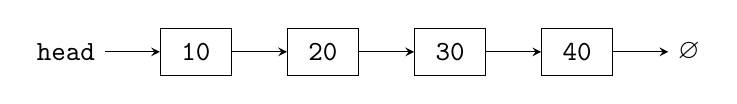
\begin{tikzpicture}[>=stealth, node distance=7mm,
    box/.style={draw, minimum width=9mm, minimum height=6mm, font=\ttfamily}]
  \node[font=\ttfamily] (head) {head};
  \node[box, right=of head] (n10) {10};
  \node[box, right=of n10]  (n20) {20};
  \node[box, right=of n20]  (n30) {30};
  \node[box, right=of n30]  (n40) {40};
  \node[right=of n40]       (nil) {$\varnothing$};
  \draw[->] (head) -- (n10);
  \draw[->] (n10)  -- (n20);
  \draw[->] (n20)  -- (n30);
  \draw[->] (n30)  -- (n40);
  \draw[->] (n40)  -- (nil);
\end{tikzpicture}
\end{center}
Then this code runs:
\begin{lstlisting}
Node p = head.next;
Node q = p.next;
p.next = q.next;
q.next = head;
head = q;
p = new Node(25, p.next);
head.next.next.next = p;
\end{lstlisting}
\begin{enumerate}
  \item Draw the final list, starting at \code{head}, as boxes and arrows.
        \score{3}
  \vspace{5cm}
  \item Which node does \code{p} refer to at the end? Which node does
        \code{q} refer to? \score{1}
  \vspace{5cm}
  \item What does a loop that prints every value from \code{head} to the
        end of the list output? \score{1}
  \vspace{5cm}
  \item Is any node unreachable (and therefore eligible for garbage
        collection) when the code finishes? Explain briefly. \score{1}
  \vspace{5cm}
\end{enumerate}

\question[18\baselineskip]{D2}{Cost of list operations}{5}
\begin{enumerate}
  \item Fill in the worst-case running time ($\Theta$) of each operation on
        a singly linked list holding $n$ elements. ``Head only'' keeps just
        a \code{head} reference; ``Head + tail'' keeps both \code{head} and
        \code{tail} references. Neither version stores a size counter.
        (4 marks: 0.5 per cell, scored by row.)
        \begin{center}
        \renewcommand{\arraystretch}{1.5}
        \begin{tabular}{|l|C{3.2cm}|C{3.2cm}|c|}
          \hline
          \textbf{Operation} & \textbf{Head only} & \textbf{Head + tail}
            & \textbf{Score} \\ \hline
          Insert at front   & & & \cellscore{1} \\ \hline
          Insert at back    & & & \cellscore{1} \\ \hline
          Remove from front & & & \cellscore{1} \\ \hline
          Remove from back  & & & \cellscore{1} \\ \hline
        \end{tabular}
        \end{center}
  \item In one sentence, explain your entry for ``Remove from back'' in the
        ``Head + tail'' column. \score{1}
\end{enumerate}

\question[18\baselineskip]{D3}{Reversing a list}{7}
\begin{enumerate}
  \item Write \code{static Node reverse(Node head)}, which reverses a singly
        linked list \textbf{in place} (by relinking nodes, not by copying
        data or creating new nodes) and returns the new head. It must run in
        $\Theta(n)$ time, use $\Theta(1)$ auxiliary space, and work for empty
        and one-node lists. \score{4}
  \vspace{5cm}
  \item A classmate wrote the recursive version below. What is its auxiliary
        space complexity, and why does it differ from your answer to (a)?
        \score{2}
\begin{lstlisting}
static Node reverseRec(Node head) {
    if (head == null || head.next == null) return head;
    Node rest = reverseRec(head.next);
    head.next.next = head;
    head.next = null;
    return rest;
}
\end{lstlisting}
\vspace{3cm}
  \item In \code{reverseRec}, which node does \code{head.next} refer to when
        the line \code{head.next.next = head;} runs, and why does that line
        put \code{head} in the right place? \score{1}
\end{enumerate}

% ================================================================ PART E
\partheading[24\baselineskip]{E}{Doubly Linked Lists}{18}

Use the \code{DNode} class from the Appendix:
\begin{lstlisting}
class DNode {
    int   data;
    DNode prev, next;
    DNode(int data) { this(data, null, null); }
    DNode(int data, DNode prev, DNode next) {
        this.data = data; this.prev = prev; this.next = next;
    }
}
\end{lstlisting}
The list uses two \textbf{sentinel} (dummy) nodes, \code{header} and
\code{trailer}, which hold no data. The first real element is
\code{header.next} and the last is \code{trailer.prev}.

\question[9\baselineskip]{E1}{Sentinels}{4}
\begin{enumerate}
  \item Draw the empty list, showing all four reference fields (\code{prev}
        and \code{next}) of \code{header} and \code{trailer}. \score{1}
  \vspace{4cm}
  \item Draw the list holding A, B, C (in that order), showing every
        \code{prev} and \code{next} reference. \score{1}
  \vspace{4cm}
  \item Give two concrete advantages of sentinel nodes. Each advantage must
        refer to a specific operation. \score{2}
  \vspace{3cm}
\end{enumerate}

\question[10\baselineskip]{E2}{$\Theta(1)$ insertion and removal}{8}
\begin{enumerate}
  \item Write \code{void insertAfter(DNode p, int x)}, which inserts a new
        node holding \code{x} immediately after node \code{p}. \code{p} may
        be \code{header} but is never \code{trailer}. It must run in
        $\Theta(1)$ time. \score{4}
  \vspace{6cm}
  \item Write \code{int remove(DNode p)}, which unlinks node \code{p} (never
        a sentinel) from the list and returns the value it held. It must run
        in $\Theta(1)$ time. \score{3}
  \vspace{6cm}
  \item Using only \code{insertAfter}, write one-line bodies for
        \code{pushFront(int x)} and \code{pushBack(int x)}. \score{1}
  \vspace{5cm}
\end{enumerate}

\question[22\baselineskip]{E3}{Find the bug}{6}
A student wrote:
\begin{lstlisting}
void insertAfterBuggy(DNode p, int x) {
    DNode q = new DNode(x);
    p.next = q;          // line 1
    q.prev = p;          // line 2
    q.next = p.next;     // line 3
    p.next.prev = q;     // line 4
}
\end{lstlisting}
The list is shown below (upper arrows are \code{next} references, lower
arrows are \code{prev} references). The student calls
\code{insertAfterBuggy(p, 7)}, where \code{p} refers to the node holding 4.
\begin{center}
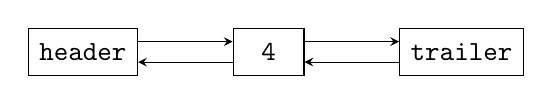
\begin{tikzpicture}[>=stealth, node distance=12mm,
    box/.style={draw, minimum height=6mm, inner sep=4pt, font=\ttfamily}]
  \node[box]                                  (hd) {header};
  \node[box, right=of hd, minimum width=9mm]  (n4) {4};
  \node[box, right=of n4]                     (tr) {trailer};
  \foreach \a/\b in {hd/n4, n4/tr} {
    \draw[->] ([yshift=1.3mm]\a.east)  -- ([yshift=1.3mm]\b.west);
    \draw[->] ([yshift=-1.3mm]\b.west) -- ([yshift=-1.3mm]\a.east);
  }
\end{tikzpicture}
\end{center}
\begin{enumerate}
  \item Draw the structure after the call. Show both references of the node
        holding 4, of the new node, and of \code{trailer}. \score{2}
  \vspace{6cm}
  \item What happens when the list is printed by following \code{next}
        references from \code{header}? What happens when it is printed
        backwards by following \code{prev} references from \code{trailer}?
        \score{2}
  \vspace{6cm}
  \item Rewrite the method so that it is correct. \score{2}
  \vspace{4cm}
\end{enumerate}

% ================================================================ PART F
\partheading[34\baselineskip]{F}{Stacks}{17}

Where a question allows it, you may use a Java stack: \code{Deque<T>}
(implemented by \code{ArrayDeque<T>}) or \code{Stack<T>}. Both provide
\code{push}, \code{pop}, \code{peek}, \code{isEmpty} and \code{size} (see
the Appendix).

\question[28\baselineskip]{F1}{Stack trace}{4}
Starting from an empty stack $S$, perform the operations below in order. As
in Java, \code{pop()} removes and returns the top element, and \code{peek()}
returns it without removing it. After each operation, write the value
returned (if any) and the contents of $S$ from bottom to top. \score{4}
\begin{center}
\renewcommand{\arraystretch}{1.4}
\begin{tabular}{|c|l|C{2.4cm}|L{6.4cm}|}
  \hline
  \textbf{\#} & \textbf{Operation} & \textbf{Returned}
    & \textbf{$S$ (bottom $\to$ top)} \\ \hline
  1  & \code{push(5)} & & \\ \hline
  2  & \code{push(3)} & & \\ \hline
  3  & \code{pop()}   & & \\ \hline
  4  & \code{push(8)} & & \\ \hline
  5  & \code{push(1)} & & \\ \hline
  6  & \code{peek()}  & & \\ \hline
  7  & \code{pop()}   & & \\ \hline
  8  & \code{push(4)} & & \\ \hline
  9  & \code{pop()}   & & \\ \hline
  10 & \code{pop()}   & & \\ \hline
  11 & \code{push(9)} & & \\ \hline
  12 & \code{size()}  & & \\ \hline
\end{tabular}
\end{center}

\question[12\baselineskip]{F2}{Which outputs are possible?}{2}
The integers 1, 2, 3, 4, 5 are pushed onto an initially empty stack
\textbf{in increasing order}. Pops may happen at any time between pushes,
every popped value is printed immediately, and all five values are
eventually popped.

For each output sequence below, say whether it is possible. If it is, give
the full sequence of operations (for example, ``push 1, push 2, pop,
\ldots''). If it is not, explain precisely why. (0.5 marks each.)
\begin{enumerate}
  \item \code{3 2 1 5 4} \score{0.5}
  \vspace{4cm}
  \item \code{4 2 3 1 5} \score{0.5}
  \vspace{4cm}
  \item \code{2 4 3 5 1} \score{0.5}
  \vspace{4cm}
  \item \code{1 5 2 4 3} \score{0.5}
\end{enumerate}

\question[15\baselineskip]{F3}{Balanced brackets}{5}
\begin{enumerate}
  \item Write \code{static boolean isBalanced(String s)}, which returns
        \code{true} exactly when the brackets \code{()}, \code{[]} and
        \code{\lb\rb} in \code{s} are properly matched and nested. Ignore
        every other character. Use a stack of \code{Character} values
        (\code{Deque<Character>} or \code{Stack<Character>}). \score{4}
        \begin{center}
        \begin{tabular}{ll}
          \toprule
          \textbf{Input} & \textbf{Result} \\
          \midrule
          \code{\lb[()()]\rb} & \code{true}  \\
          \code{a(b[c]d)e}    & \code{true}  \\
          \code{([)]}         & \code{false} \\
          \code{((}           & \code{false} \\
          \code{())}          & \code{false} \\
          \bottomrule
        \end{tabular}
        \end{center}
  \vspace{8cm}
  \item Give the time and auxiliary space complexity of your function for a
        string of length $n$, and describe an input that needs the most
        space. \score{1}
\end{enumerate}

\question[11\baselineskip]{F4}{Expressions}{6}
\begin{enumerate}
  \item Evaluate the postfix expression below using a stack. Show the stack
        (bottom $\to$ top) after \textbf{each} token is processed. All
        operators are binary, and \code{/} is integer division. \score{3}
        \begin{center}\code{8 2 5 * + 1 3 2 * + 4 - /}\end{center}
 \vspace{9cm}
  \item Convert the infix expression below to postfix using the
        operator-stack (shunting-yard) algorithm. After each token, show the
        output so far and the operator stack. \code{*} and \code{/} have
        higher precedence than \code{+} and \code{-}, and all four operators
        are left-associative (i.e., the compiler starts processing from the left). \score{3}
        \begin{center}\code{A + B * ( C - D ) / E}\end{center}
\end{enumerate}

% ================================================================ PART G
\partheading[28\baselineskip]{G}{Queues}{6}

\question{G1}{A linked queue}{6}
Implement a queue of integers with a singly linked list of \code{Node}s (see
the Appendix), keeping both a \code{head} and a \code{tail} reference so
that \code{enqueue} and \code{dequeue} both run in $\Theta(1)$ time.
\begin{lstlisting}
public class LinkedQueue {
    private Node head = null;
    private Node tail = null;

    public void enqueue(int x) { /* your code */ }

    // Throws NoSuchElementException if the queue is empty.
    public int dequeue()       { /* your code */ }

    public boolean isEmpty()   { return head == null; }
}
\end{lstlisting}
\begin{enumerate}
  \item Which end of the list must be the \textbf{front} of the queue (where
        \code{dequeue} happens)? Explain why the other choice cannot give
        $\Theta(1)$ for both operations. \score{1}
  \vspace{6cm}
  \item Write \code{enqueue} and \code{dequeue}. Pay particular attention to
        enqueuing into an empty queue and to dequeuing the last element.
        \score{5}
\end{enumerate}

% ================================================================ PART H
\partheading[26\baselineskip]{H}{The Function Call Stack}{5}

\question{H1}{Stack frames and the heap}{5}
\begin{enumerate}
  \item List four kinds of information stored in a method's stack frame
        (i.e., activation record). \score{2}
  \vspace{3cm}
  \item Consider:
\begin{lstlisting}
static int[] build(int n) {
    int total = 0;
    Node temp = new Node(42);
    int[] arr = new int[n];
    for (int i = 0; i < n; i++) {
        arr[i] = i;
        total += i;
    }
    return arr;
}
\end{lstlisting}
        For each of (i) \code{total}, (ii) the reference variable \code{arr}
        itself, (iii) the $n$-element array that \code{arr} refers to, and
        (iv) the \code{Node} object that \code{temp} refers to, say whether
        it lives on the \textbf{call stack} or on the \textbf{heap}, and what
        happens to it after \code{build} returns. \score{2}
  \vspace{5cm}
  \item A classmate claims: ``\code{arr} is a local variable, so the array
        is destroyed when \code{build} returns and the caller receives
        garbage.'' Explain what is wrong with this claim. \score{1}
\end{enumerate}

% ================================================================ PART I
\partheading[22\baselineskip]{I}{Design Problems}{8}

\question{I1}{A stack with a minimum}{8}
Design a stack of integers that supports \code{push(x)}, \code{pop()}
(remove and return the top value), \code{peek()} and \code{getMin()} (return
the smallest value currently in the stack), \textbf{each in $\Theta(1)$
time}: worst case for \code{pop}, \code{peek} and \code{getMin}, and
amortized for \code{push}, because the library stacks' \code{push} is
amortized $\Theta(1)$ (see the Appendix).
\begin{enumerate}
  \item Describe your idea in two to four sentences. \score{2}
  \vspace{7cm}
  \item Write the class in Java. You may use \code{Deque<Integer>} (with
        \code{ArrayDeque}) or \code{Stack<Integer>}, and you may assume
        \code{pop}, \code{peek} and \code{getMin} are never called on an
        empty stack. \score{4}
  \vspace{8cm}
  \item How much auxiliary space does your design use in the worst case?
        Give an input that reaches it. \score{1}
  \vspace{8cm}
  \item Trace your design on: \code{push(5)}, \code{push(3)},
        \code{push(7)}, \code{push(3)}, \code{pop()}, \code{getMin()},
        \code{pop()}, \code{pop()}, \code{getMin()}. Give the value returned
        by each \code{getMin()}. \score{1}
\end{enumerate}

% ============================================================== APPENDIX
\clearpage
\section*{Appendix --- Reference Sheet}

\subsection*{Node classes}
\begin{lstlisting}
class Node {                     // singly linked
    int  data;
    Node next;
    Node(int data)            { this(data, null); }
    Node(int data, Node next) { this.data = data; this.next = next; }
}

class DNode {                    // doubly linked
    int   data;
    DNode prev, next;
    DNode(int data) { this(data, null, null); }
    DNode(int data, DNode prev, DNode next) {
        this.data = data; this.prev = prev; this.next = next;
    }
}
\end{lstlisting}
Assume \code{import java.util.*;} at the top of every file.

\subsection*{Java library interfaces}
\begin{center}
\small
\renewcommand{\arraystretch}{1.25}
\begin{tabularx}{\textwidth}{@{}l Y l Y@{}}
  \toprule
  \multicolumn{2}{@{}l}{\textbf{Stack:} \code{Deque<T> s = new ArrayDeque<>();}}
    & \multicolumn{2}{l@{}}{\textbf{Queue:} \code{Queue<T> q = new ArrayDeque<>();}} \\
  \cmidrule(r){1-2}\cmidrule(l){3-4}
  \code{s.push(x)}   & add \code{x} on top
    & \code{q.offer(x)}  & add \code{x} at the back \\
  \code{s.pop()}     & remove and return the top
    & \code{q.poll()}    & remove and return the front (\code{null} if empty) \\
  \code{s.peek()}    & return the top without removing it
    & \code{q.peek()}    & return the front without removing it \\
  \code{s.isEmpty()} & \code{true} if empty
    & \code{q.isEmpty()} & \code{true} if empty \\
  \code{s.size()}    & number of elements
    & \code{q.size()}    & number of elements \\
  \bottomrule
\end{tabularx}
\end{center}
\begin{itemize}
  \item \code{java.util.Stack<T>} offers the same five stack methods.
        Calling \code{pop()} on an empty stack throws an exception.
  \item Collections store objects, so \code{int} values are automatically
        boxed to \code{Integer} and unboxed back.
  \item Each operation above runs in $\Theta(1)$ time (amortized
        $\Theta(1)$ for \code{push} and \code{offer}).
\end{itemize}

\end{document}